\section{Case Studies}
\label{sec:test}
In this section, we present two recognition SNN models working on the Poissonian subset of the NE15-MNIST dataset.
Their network components, training and testing methods are described according to the evaluation methodology stated above.
The specific spike-based evaluations on input event rates and responding latency are also provided. 
Meanwhile, as tentative benchmarks the models are implemented on SpiNNaker to assess the performance against software simulators.
Presenting proper benchmarks for vision recognition systems is still under investigation, the case studies only make an attempt.

\subsection{Case Study I}
The first case study is a simple two-layered network where the input neurons receive Poissonian presented spike trains from the dataset and form a fully connected (FC) network with the decision neurons.
The model utilises Leaky-Integrate-and-Fire (LIF) neurons, and the parameters are all with biological means, see the listed values in Table~\ref{tbl:pynnSetting}.
The connections between the input neurons and the decision neurons are plastic, so the connection weights can be modulated during training with standard STDP learning rule.
The model is described with PyNN and the code is published in\footnote {https://github.com/qian-liu/benchmarking/tree/master/code/case\_study\_I} the same github repository with the dataset.
Considering to be a potential benchmark, this system is composed with simple neural models, trained with standard learning rules and written in a unified SNN description language. These characteristics allow the same network on to be tested on various simulators, both software- and hardware-based.
%Consequently, the benchmark can be directly run on different SNN simulators as long as PyNN is supported.
%Besides, any modification on neuron or learning model is not required since only standard models are used.
%During training, each decision neuron is triggered by a teaching neuron while the weights of the synaptic connections of the input neurons and the decision neuron are modulated with standard STDP learning rule, see Fig~\ref{Fig:train}.

Both the training and testing exploit the Poissonian subset of the NE15-MNIST dataset.
Because different simulators generate random Poissonian spike trains with various mechanisms, languages and codes, using the same dataset enables   performance evaluation of these simulators without the interference created by non-unified input.
In terms of this case study, the performance of the model was evaluated with both software simulation (on NEST~\citep{gewaltig2007nest}) and hardware implementation (on SpiNNaker).

In order to fully assess the performance, different settings have been configured on the network, such as network size, input rate and testing images duration.
For simplicity of describing the system, one standard configuration is set as example in the following sections.
\begin{table}[hbbp]
\centering
\caption{\label{tbl:pynnSetting}Parameter setting for the current-based LIF neurons using PyNN.}
\bgroup
\def\arraystretch{1.1}
  \begin{tabular}{c|c|c}
  %\hline
  Parameters & Values & Units \\
  \hline
  cm & 0.25 & nF	\\
  %\hline
  tau\_m & 20.0 & ms\\
  %\hline
  tau\_refrac & 2.0 & ms\\
  %\hline
  tau\_syn\_E & 1.0 & ms\\
  %\hline
  tau\_syn\_I & 1.0 & ms\\
  %\hline
  v\_reset & -70.0 & mV\\
  %\hline
  v\_rest & -65.0 & mV\\
  %\hline
  v\_thresh & -50.0 & mV\\
  %\hline
  \end{tabular}
\egroup
\end{table}

%\subsection{Description of the data used}
\subsubsection{Training}

There are two layers in the model: 28$\times$28 input neurons fully connect to 100 decision neurons.
Each decision neuron responds to a certain template of a digit.
In the standard configuration, there are 10 decision neurons answering to the same digit with slightly different templates.
Those templates are embedded in the connection weights between the two layers.
Fig~\ref{Fig:train} shows how the connections to a single decision neuron is tuned.

The training set of $60,000$ hand written digits are firstly classified into 100 classes, 10 subclasses per digit, using K-means clusters.
So the images in a certain subclass are used to train one corresponding decision neuron.
The firing rate of the input neurons are assigned linearly according to their intensities and normalised with a total firing rate of 2000~Hz.
All the images together are presented 180~$s$ (about 300~$ms$ per image) during training and at the same time a teaching signal of 50~Hz is conveyed to the decision neuron to trigger STDP learning.
The trained weights are plotted in accordance with the positions of the decision neurons in Fig~\ref{Fig:test}.
\begin{figure}[thb!]
	\centering
	\subfloat[Training model of a single decision neuron.]{
		\label{Fig:train}
		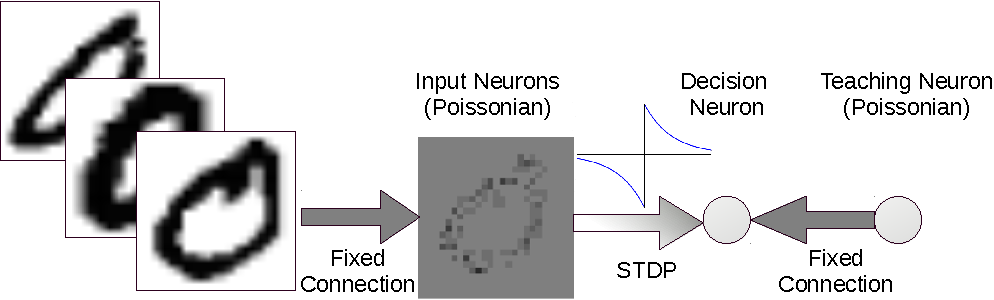
\includegraphics[width=0.48\textwidth]{images/training.pdf}
		} \\

	\centering
	
	\subfloat[Testing model of the spiking neural network.]{
		\label{Fig:test}
		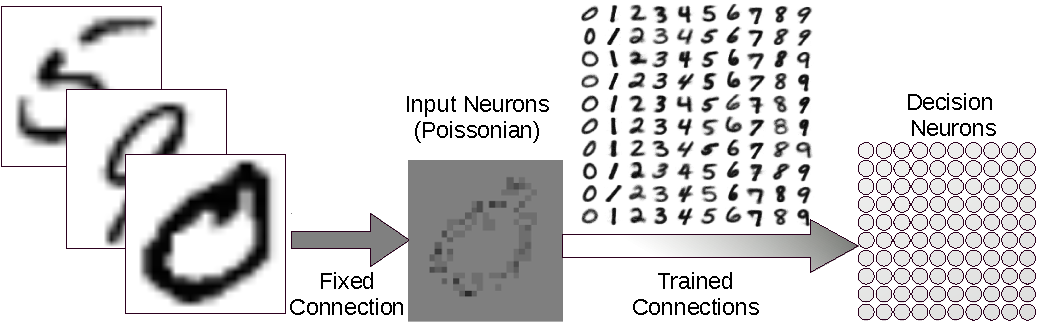
\includegraphics[width=0.48\textwidth]{images/testing.pdf}
		}
		
	\caption{The training and testing model of the two-layered spiking neural network.}
	\label{fig:model}
\end{figure} 



\subsubsection{Testing}
After training the weights of the plastic synapses are set to static, keeping the state of the weights on the last moment during training.
%The weights were normalised after training and applied to the same network.
And the weak weights were set to inhibitory connections with an identical strength.
%The output neurons inhibited all the other neurons as a winner take all circuit.
The feed-forward testing network is shown in Fig~\ref{Fig:test} where Poissonion spike trains are generated the same way as in the training with a total firing rate of 2000~Hz per image.
The input neurons convey the same spike trains to every decision neuron through its responding trained synaptic weights. 
Every testing image ($10,000$ images in total) is presented once and lasts 1 second with a silence of 200~ms between them.
The output neuron with the highest firing rate decides what digit was recognized.
Taken the trained weights from NEST simulation, the accuracy of the recognition on NEST as well reaches 89.94\% with the standard configuration, while the result drops slightly to 89.88\% using SpiNNaker.
In comparison, trained and tested both on SpiNNaker the recognition accuracy is 87.41\%, and the same weights applied to NEST the result turns to be 87.25\%. 
%In order to compare the recognition difference, another experiment on SpiNNaker is taken to test with the same NEST trained weights.
The recording of the output neurons of a test sequence of digits is shown in the raster plot (Fig~\ref{Fig:output}).
In order to make the raster plot easier to read, we apply inhibit connections between neurons which are not in the same subclasses.


\begin{figure}[hbt!]
	\centering
	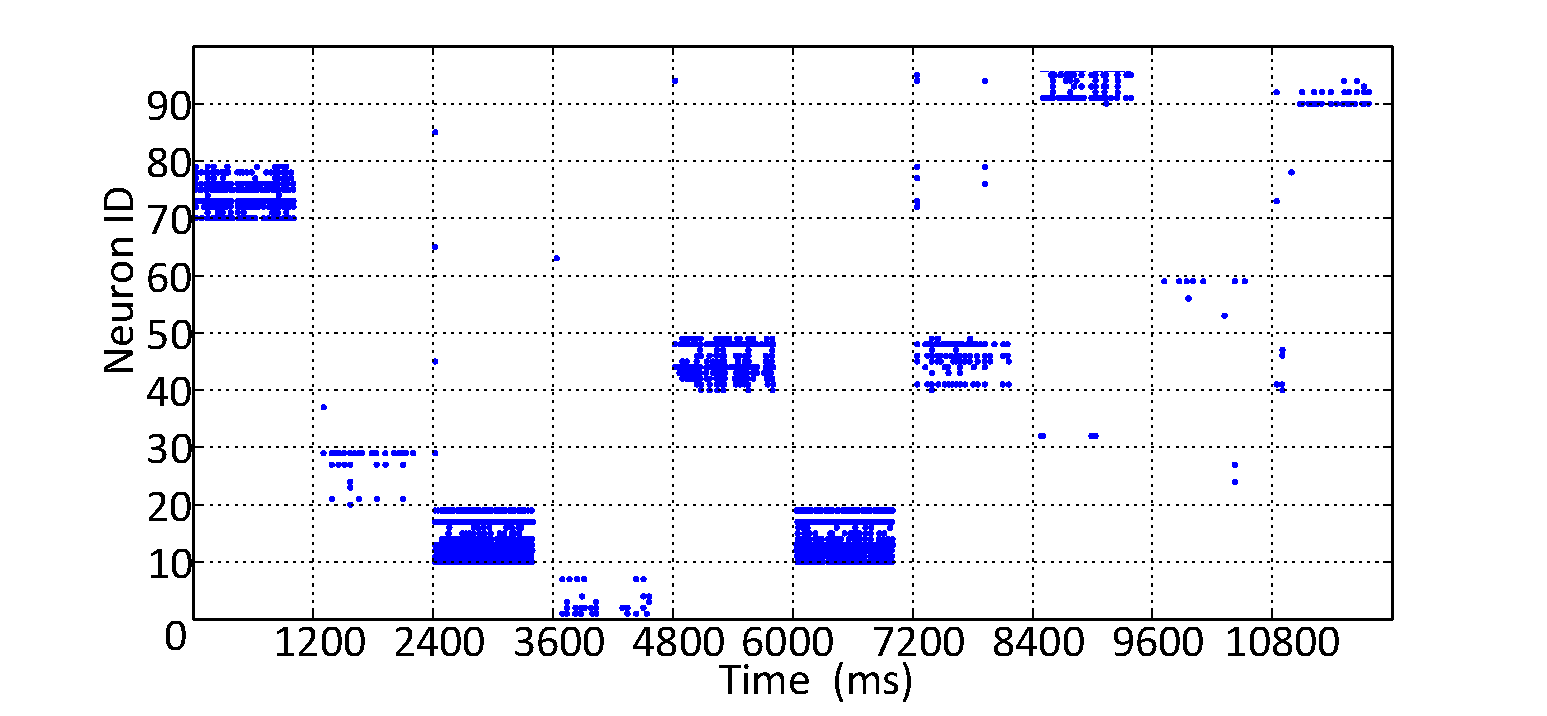
\includegraphics[width=0.48\textwidth]{images/decision.pdf}
	\caption{A raster plot of spike trains of the decision neurons. The sequence of the testing images are (7, 2, 1, 0, 4, 1, 4, 9, 5, 9).}
	\label{Fig:output}
\end{figure} 
\subsubsection{Evaluation}
The evaluation starts from the hardware-independent side, focusing on the spike-based recognition analysis.
As mentioned in Section~\ref{subsec:model}, classification accuracy (CA) and response time (latency) are the main concerns assessing the recognition capability.
In our experiment, two sets of weights were applied: original STDP trained weights and scaled-up weights which are 10 times stronger. Spiking rates of testing samples were also modified, ranging from 10 to 5000~Hz.

We found that accuracy depends largely on the time each sample is exposed to the network and the sample spiking rate (Fig.~\ref{fig:assess}.)
Furthermore, the latency of the output of the decision neurons is affected by both the spiking rate and connection weights.
Fig.~\ref{fig:acc_time} shows that the CA is better as exposure time increases. The longer an image is presented, the more information is gathered by the network, so the accuracy climbs.
Classification accuracy also increases when input spiking rates are augmented (Fig.~\ref{fig:acc_rate}.) Given that the spike trains injected into the network are more intense, the decision neurons become more active and so does the output disparity among them.
Nonetheless, it is important to know that these increments in CA have a limit, as is shown in the aforementioned figures.
%However, with increasing spikes injected the spiking rate of the decision neurons saturate to the limit of $1/tau\_refrac$, where $tau\_refrac$ refers to the refractory period.  
%So, the rate gap between the correct decision neuron and the others narrow as the input rates increase to a certain level.
With stronger weights, the accuracy is much higher when the input firing rate is less than 2000~Hz.


The latency of a SNN model is the result of the input rates and synaptic weights.
As the input rates grow, there are more spikes arriving at the decision neurons, triggering them to spike sooner.
A similar idea applies to the influence of synaptic weights. If stronger weights are taken, then the membrane potential of a neuron reaches its threshold earlier.
Fig.~\ref{fig:lat_rate} indicates the latency is shortened with increasing input rates with both the original and scaled-up weights.
When the spiking rate is less than 2000~Hz, the network with stronger weights has a much shorter latency.
As long as there are enough spikes to trigger the decision neurons to spike, increasing the test time will not make the network respond sooner~(Fig.~\ref{fig:lat_time}.)
	\begin{figure}[htb!]
	  \centering
	  \subfloat[Accuracy changes against test time.]{
	  	    \label{fig:acc_time}
	  	    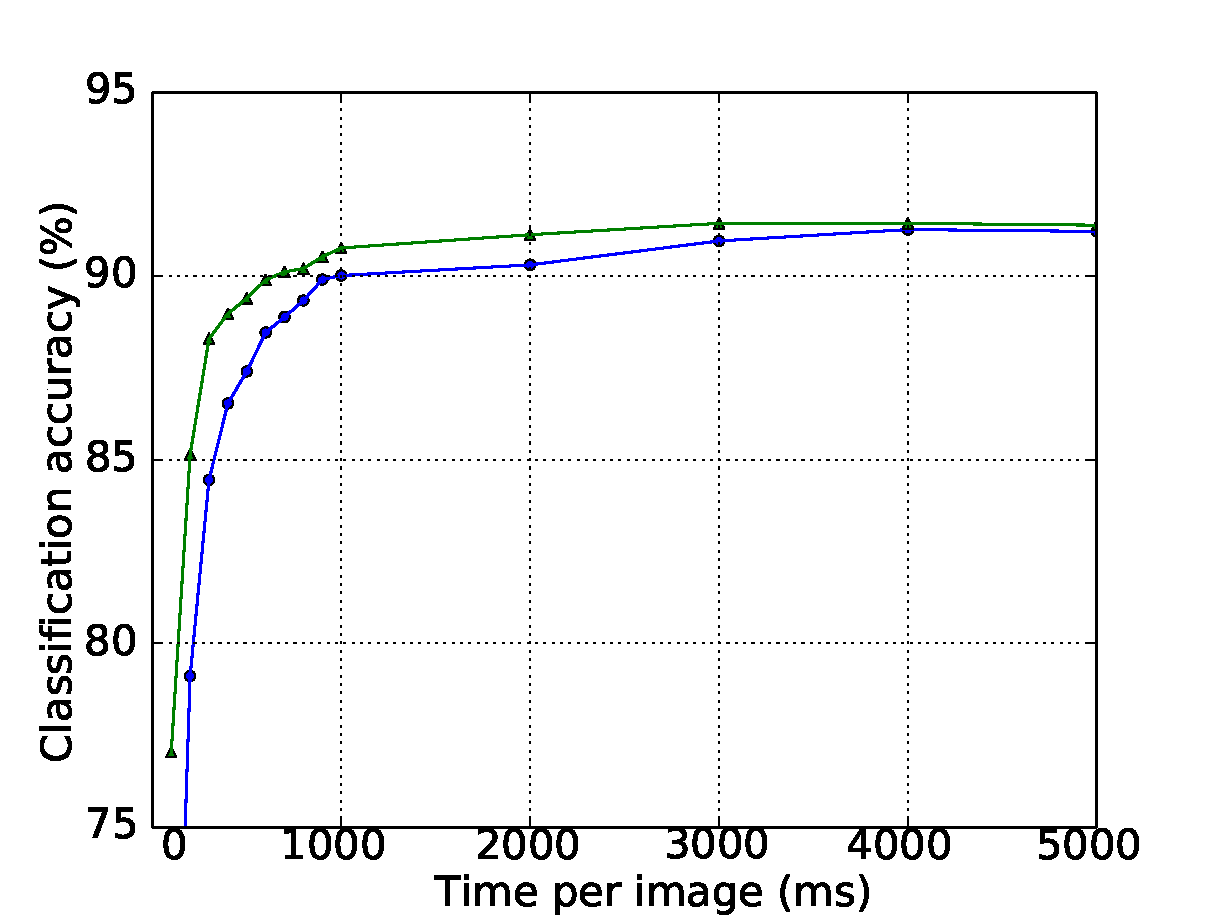
\includegraphics[width=0.25\textwidth]{acc_dur.pdf}
	  	  }
	  \subfloat[Accuracy changes against firing rate.]{
	  	    \label{fig:acc_rate}
	  	    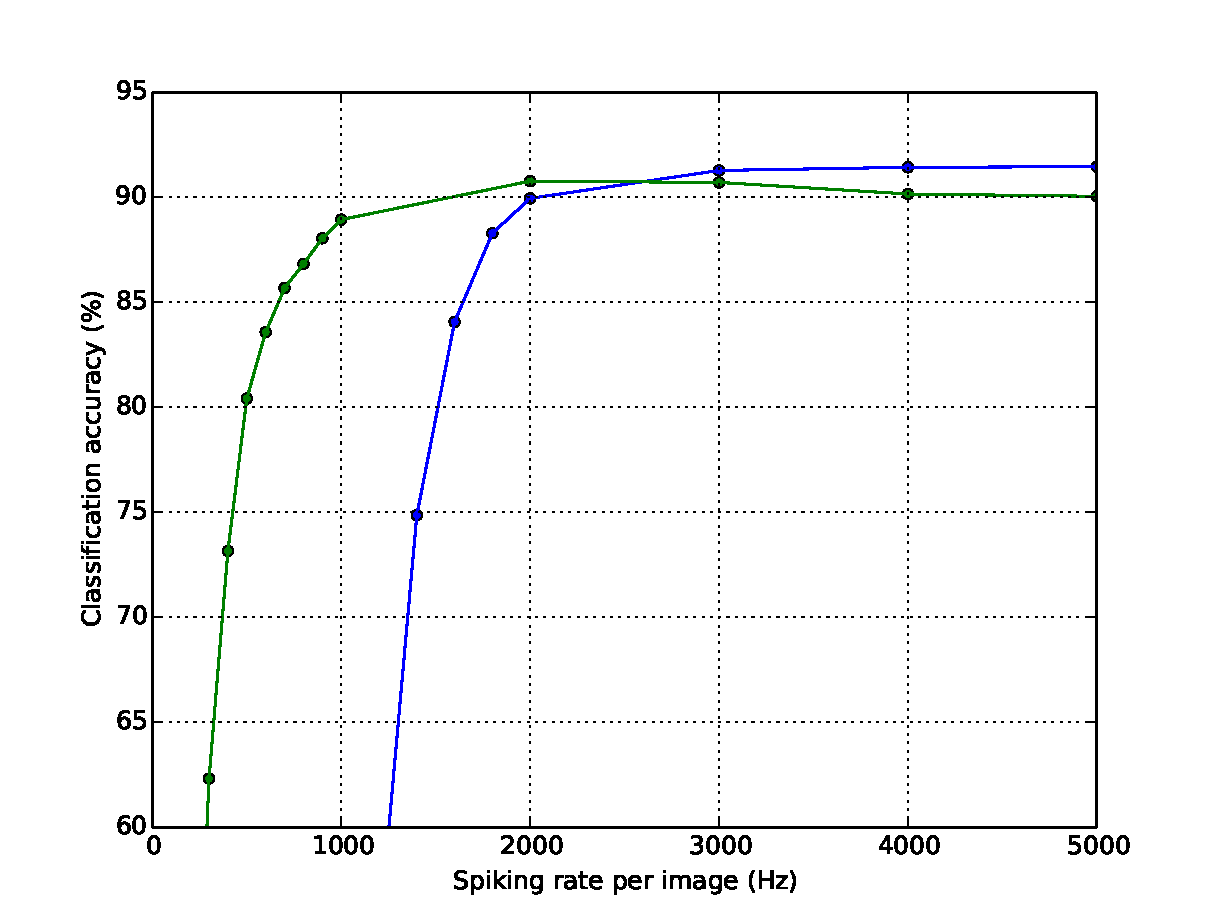
\includegraphics[width=0.25\textwidth]{acc_rate.pdf}
	  	  }
	  	  \\
	  \subfloat[Latency stablises against test time.]{
	  	    \label{fig:lat_time}
	  	    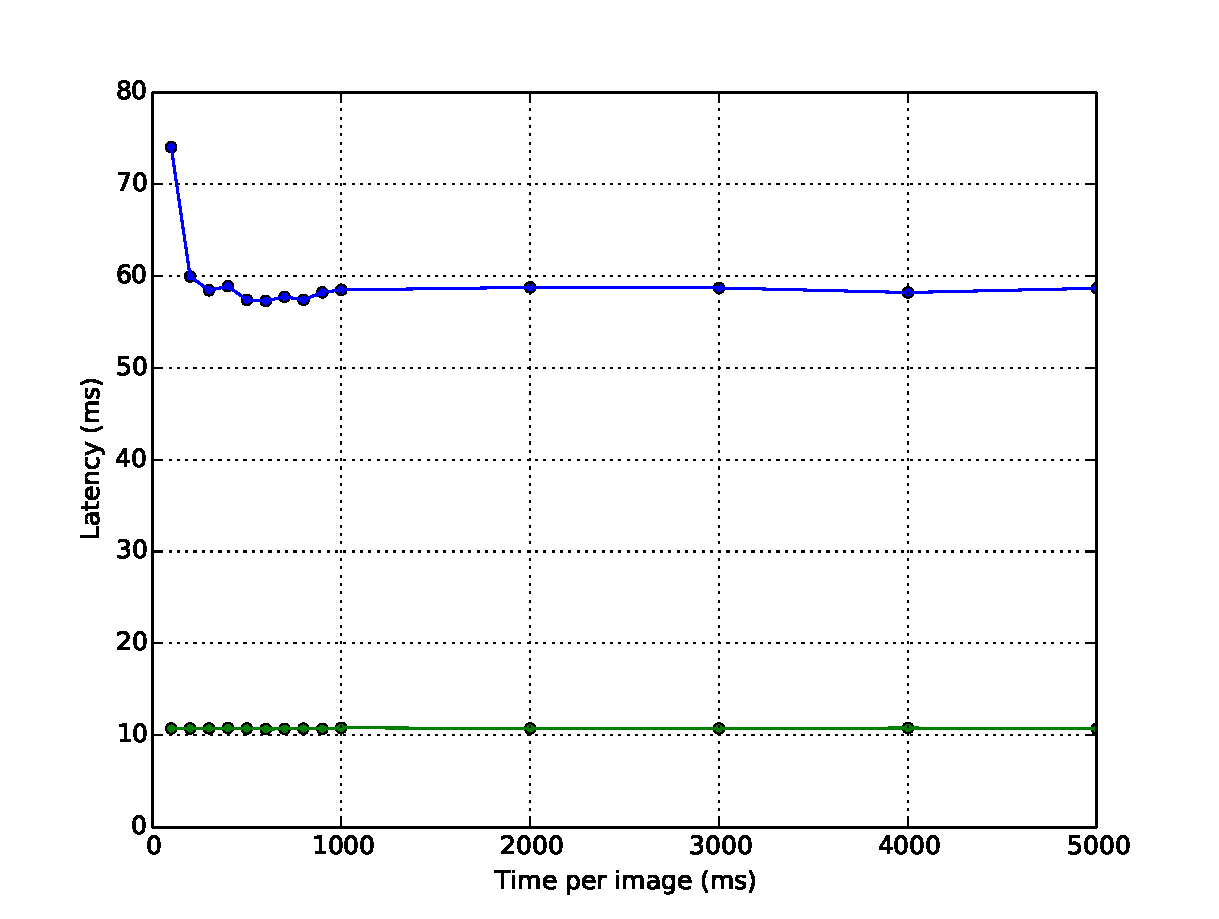
\includegraphics[width=0.25\textwidth]{lat_dur.pdf}
	  	  }
	  \subfloat[Latency changes against firing rate.]{
	  	    \label{fig:lat_rate}
	  	    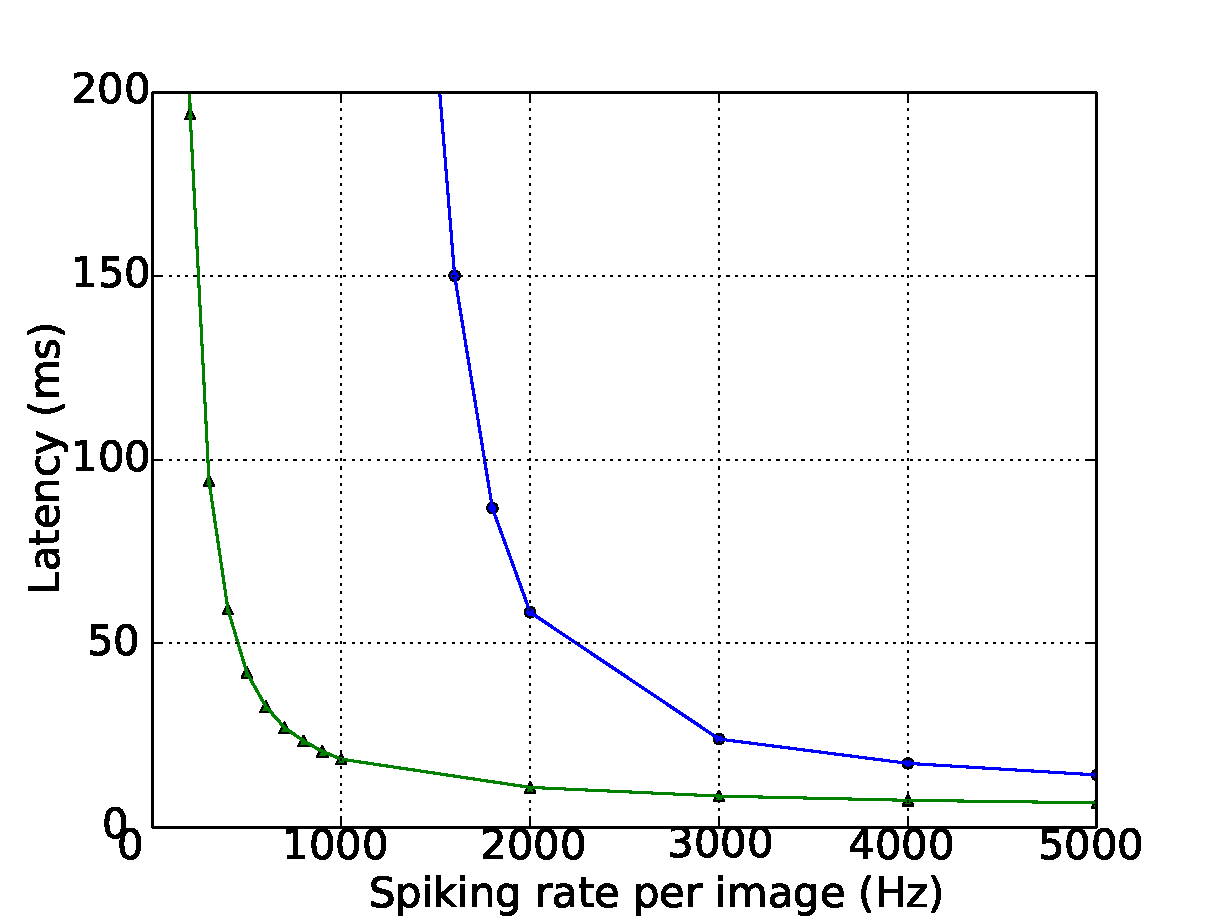
\includegraphics[width=0.25\textwidth]{lat_rate.pdf}
	  	  }
	  \caption{Accuracy and response time (latency) change over test time and input firing rate per testing image. Original trained weights are used (in blue) as well as the scaled up ($\times10$) weights (in green). }
	  \label{fig:assess}
	\end{figure}

Regarding the network size, it not only influences the accuracy of a model but also the time taken for simulation on specific platforms thus impacting the energy usage on the hardware.
For the purpose of comparing the accuracy, simulation time and energy usage, different configurations have been tested on NEST (working on a PC with CPU: i5-4570 and 8G memory) and SpiNNaker, see to Table~\ref{tbl:compare}.
The input rates of all the tests are 5000~Hz, and each image is presented 1~s.
The configurations only differ in number of templates (subclasses) per digit.
The recognition accuracies differ in a range of $\pm0.5\%$ between NEST and SpiNNaker due to the limited fast memory and the necessity for fixed-point arithmetic on SpiNNaker to ensure real-time operation.
It is inevitable that numerical precision will be below IEEE double precision at various points in the processing chain from synaptic input to membrane potential.
The main bottleneck is currently in the ring buffer where total precision for accumulated spike inputs is 16-bit, meaning that individual spikes are realistically going to be limited to 11- to 14-bit depending upon the probabilistic headroom calculated as necessary from the network configuration and spike throughput~\cite{Hopkins2015Accuracy}.
As the growth of network size there are more decision neurons and synapses connecting to them, thus the simulation time on NEST increases.
On the other hand, SpiNNaker works in real time (biology time) and the simulation time becomes shorter when 1000 patterns per digit are used.
The Thermal Design Power (TDP) usage of all four processors active operating at Base Frequency is 84~W.
Nest was run fully active on a single core which cost 21~W of power usage.
The energy use can be calculated as the product of the simulation time and the power use.
Even with the smallest network, SpiNNaker wins in the energy cost comparison, see Fig~\ref{fig:energy}.
Among different network configurations, the network of 500 decision neurons reaches the highest recognition rate.
%The recognition accuracy reaches the highest (92.98\%) when 50 patterns are trained per digit.
The network achieved the recognition accuracy of 92.98\%, average latency of 10.70~ms and energy use of 4920~J on SpiNNaker.

\begin{table}[h]
\caption{Comparisons of NEST and SpiNNaker performances.}
\begin{center}
\begin{tabular} {r|c|c|c|c|c|c}
	 Subclasses
	 &\multicolumn{2}{c|}{Accuracy (\%)}  &\multicolumn{2}{c|}{Simulation (s)}
	 &\multicolumn{2}{c}{Power Use (W)}   \\
	 \cline{2-7}
	 per digit
	& N & S & N & S & N & S\\
    \hline
    1 & 79.62 & 79.50 & 554.77 & \multirow{5}{*}{12000} & \multirow{5}{*}{ 21.0 } & 0.38 \\
    10 & 91.29 & 91.43 & 621.74 &   &   & 0.38 \\
    50 & 92.98 & 92.92 & 1125.12 &   &   & 0.41 \\
    100 & 87.27 & 86.83 & 1406.01 &   &   & 0.44 \\
    1000 & 89.65 & NA & 30316.88 &   &   & 1.50 \\

\end{tabular}
\label{tbl:compare}
\end{center}
\end{table}

\begin{figure}[hbt!]
	\centering
	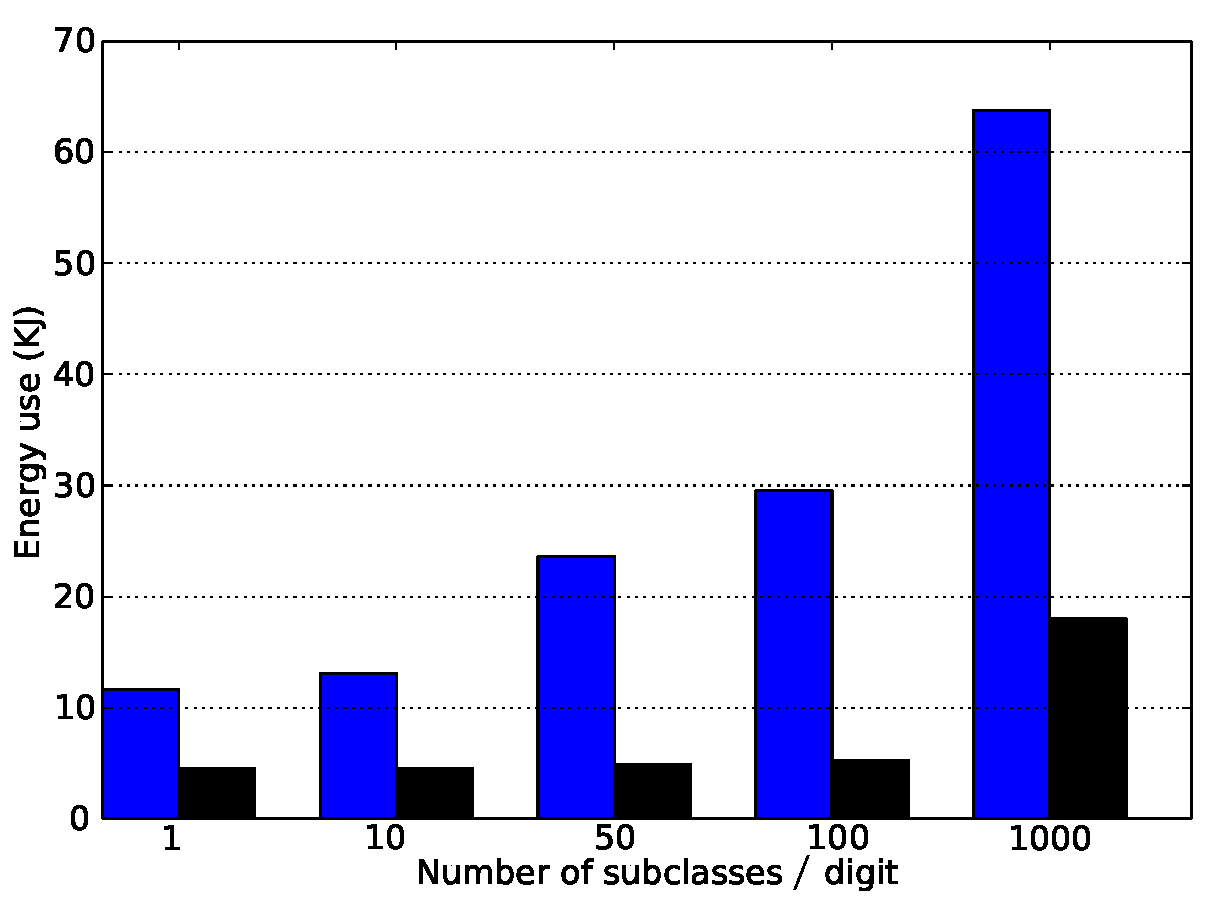
\includegraphics[width=0.48\textwidth]{images/energy.pdf}
	\caption{Energy usages of different network size both using NEST(blue) on a PC and SpiNNaker(green).}
	\label{fig:energy}
\end{figure}
\subsection{Case Study II}
% brief intro about dbn
Deep learning architectures and in particular Convolutional Networks \citep{lecun1998gradient} and Deep Belief Networks (DBNs) \citep{Hinton_etal_2006} have been characterised as one of the breakthrough technologies of the decade \citep{MIT_TechReview}. One of the advantages of these type of networks is that their performance can be increased by adding more layers \citep{Hinton_Contr_Divergence2006}.

However, state-of-the-art deep networks comprise a large number of layers, neurons and connections resulting in high energy demands, communication overheads, and high response latencies. This is a problem for mobile and robotic platforms which may have limited computational and power resources but require fast system responses. 


% about oneils model 
\citet{10.3389/fnins.2013.00178} proposed a method to map off-line trained DBNs into a spiking neural networks and take advantage of the real-time performance and energy efficiency of neuromorphic platforms. This lead initially to an implementation on an event-driven Field-Programmable Gate Array (FPGA) called Minitaur \citep{dannminitaur} and then on the SpiNNaker platform \citep{iscasSpinnakerAcceptedDemo,SpinnakerDBN2015}. For this work we used an off-line trained\footnote{\url{https://github.com/dannyneil/edbn/}} spiking DBN with a 784-500-500-10 network topology. Simulations take place on a software spiking neural network simulator named Brian \citep{briansim} and results are verified on the SpiNNaker platform.

\subsubsection{Training}

DBNs consist of stacked Restricted Boltzmann Machines (RBMs), which are fully connected recurrent networks but without any connections between neurons of the same layer. Training is performed unsupervised using the standard Contrastive Divergence (CD) rule \citep{Hinton_Contr_Divergence2006} and only the output layer is trained in a supervised manner. The main difference between spiking DBNs and traditional DBNs is the activation function used for the neurons. \citet{10.3389/fnins.2013.00178} proposed the use of the Siegert approximation \citep{Jug_etal_2012} as the activation function, which returns the expected firing rate of a leaky integrate and fire (LIF) neuron given input firing rates, input weights, and standard neuron parameters.

\subsubsection{Testing}
After the training process the learnt synaptic weights can be used in a spiking neural network which consists of LIF neurons with delta-current synapses. Table~\ref{Tab:NeuralParams} shows the LIF parameters used in the simulations.

%\begin{table}[htb!]
%\textbf{\refstepcounter{table}\label{Tab:NeuralParams} Table \arabic{table}.}{ Default parameters of the Leaky Integrate-and-Fire Model used in simulations.}
%
%\processtable{}
%{\begin{tabular}{c|c|c} %{lllll}\toprule
%Parameters & Values & Units \\
%\hline
%$\tau_{m}$ 		 & 5.0 & s  \\
%$T_{\mathrm{refract}}$ & 2.0 & ms \\
%%$V_{\mathrm{init}}$ 		 & 0.0 & mV\\
%$V_{\mathrm{reset}}$ 		 & 0.0 & mV \\
%$V_{\mathrm{thresh}}$ 		 & 1.0 & mV \\
%\end{tabular}}{}
%\end{table}
\begin{table}[hbbp]
\centering
\caption{\label{Tab:NeuralParams}Default parameters of the Leaky Integrate-and-Fire Model used in simulations.}
\bgroup
\def\arraystretch{1.1}
  \begin{tabular}{c|c|c}
  %\hline
  Parameters & Values & Units \\
  \hline
  tau\_m & 5 & s\\
  %\hline
  tau\_refrac & 2.0 & ms\\
  %\hline
  v\_reset & 0.0 & mV\\
  %\hline
  v\_rest & 0.0 & mV\\
  %\hline
  v\_thresh & 1.0 & mV\\
  %\hline
  \end{tabular}
\egroup
\end{table}

The pixels of each MNIST digit from the testing set are converted into Poisson spike trains with a rate proportional to the intensity of their pixel, while their firing rates are scaled so that the total firing rate of the input population is constant \citep{10.3389/fnins.2013.00178}.
  
The classification accuracy (CA) was chosen as the performance metric of the spiking DBN, which is the percentage of the correctly classified digits over the whole MNIST testing set.
 
%Table~\ref{tab:casimulators} presents a comparison of the classification accuracies (CA) between the rate-based implementation in MATLAB using the Siegert neurons, Brian, and SpiNNaker. %The default fixed-point weight precision for SpiNNaker is 22 bits, 6 for the integer part and 16 for the fractional part (Q6.16) \citep{}.





\subsubsection{Evaluation}

%Investigate CA as a function of weight precision
%and input firing rates for neuromorphic plaforms 
%verify brian results with spinnaker for a particular
%weight precision.

Neuromorphic platforms may have limited hardware resources to store the synaptic weights \citep{Schemmel_etal10,Merolla08082014}. In order to investigate how the precision of the weights affect the classification accuracy (CA) of a spiking DBN the double floating point weights of the offline trained network were converted to different fixed-point representations. The following notation will be used throughout this paper, Q\textit{m.f}, where \textit{m} signifies the number of bits for the integer part (including the sign bit) and \textit{f} the number of bits used for the fractional part.

Figure~\ref{Fig:brianCAfiringrate} shows the effect of reduced weight bit precision on the CA for different input firing rates on the Brian simulator. To validate the results of the software simulator simulations ran on SpiNNaker for a weight resolution of Q3.8. SpiNNaker achieved a CA of 94.94\% when 1500~Hz was used for the input population \citep{SpinnakerDBN2015,iscasSpinnakerAcceptedDemo}. Brian for the same firing rates and weight precision achieved a CA of 94.955\%. Results are summarised in Table~\ref{tab:casimulators}.   

\begin{figure}[hbt!]
	\centering
	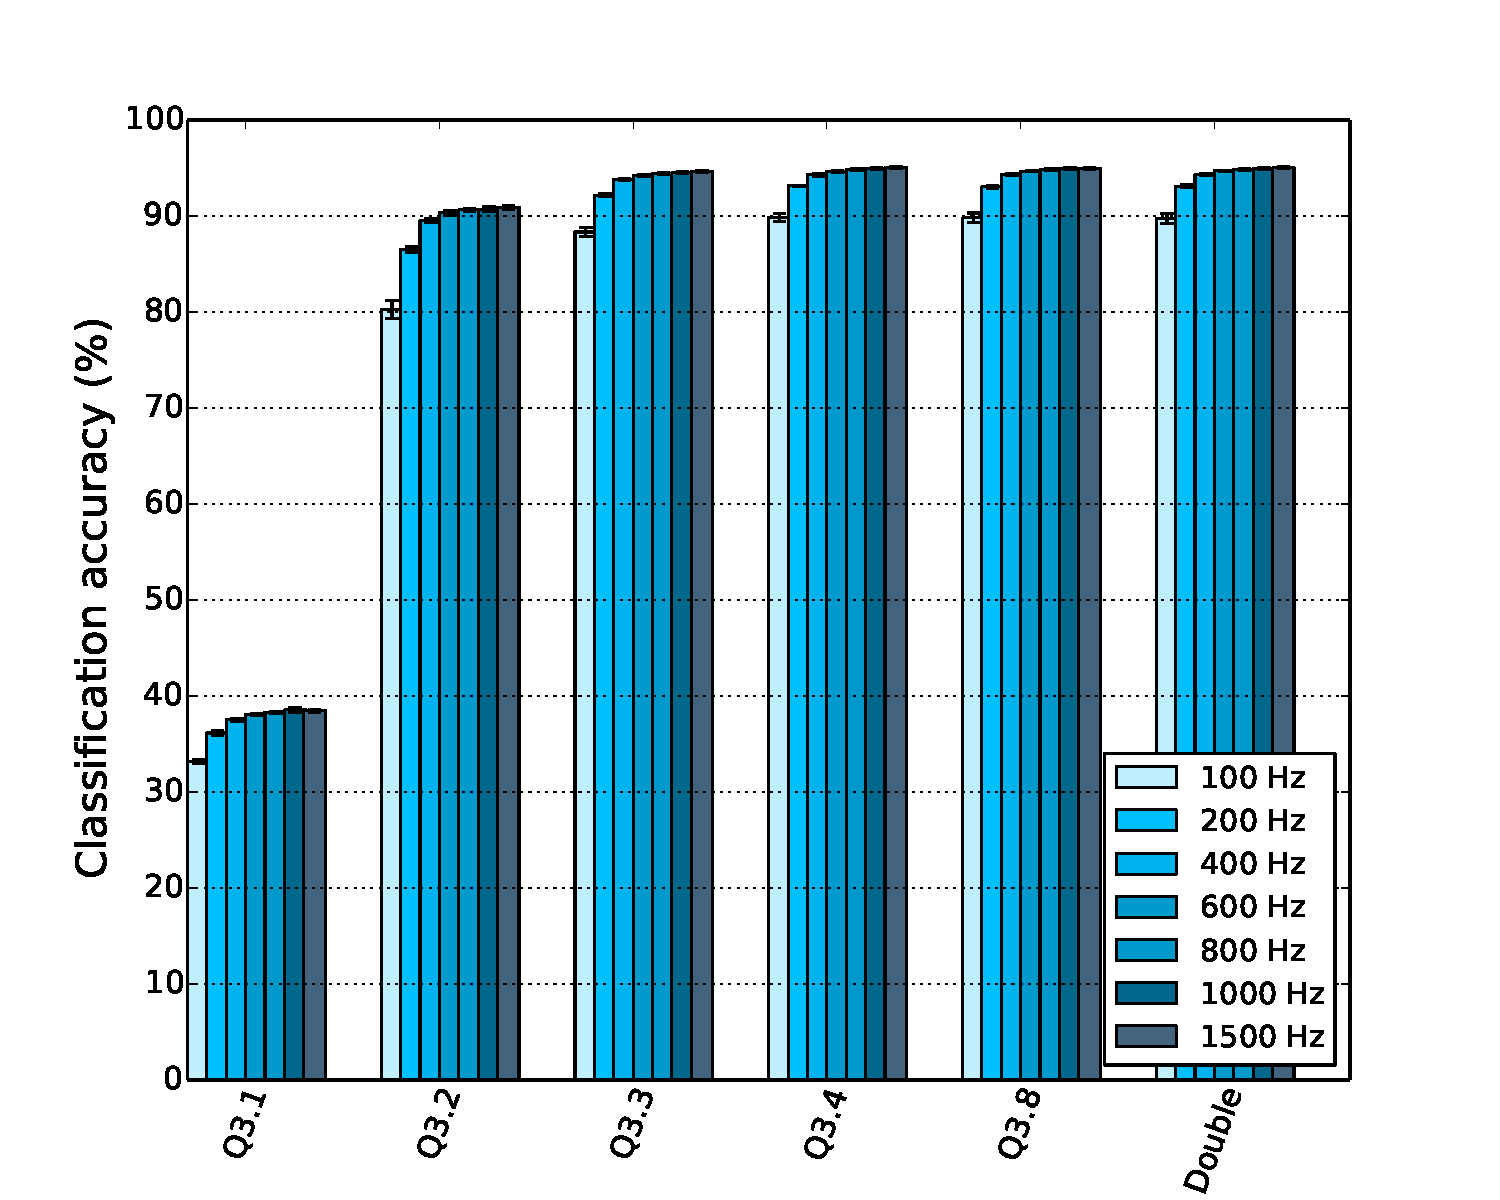
\includegraphics[width=0.48\textwidth]{images/evan/cavsfiringrate.pdf}
	\caption{CA as a function of the weight bit precision for different input firing rates.}
	\label{Fig:brianCAfiringrate}
\end{figure} 


\begin{table}[h]
\caption{Classification accuracy (CA) of the same DBN running on different platforms.}
\begin{center}
\begin{tabular} {c|c|c}
	Simulator & CA (\%) & Weight Precision \\
%    \multicolumn{1}{|c|}{\textbf{Simulator}}
%    & \multicolumn{1}{|c|}{\textbf{CA (\%)}}
%    & \multicolumn{1}{|c|}{\textbf{Weight Precision}} \\
    \hline
    Matlab & 96.06 & Double floating point\\
    Brian & 95.00 & Double floating point\\
    Brian & 94.955 & Q3.8\\
    SpiNNaker & 94.94 & Q3.8\\
%    \hline
\end{tabular}
\label{tab:casimulators}
\end{center}
\end{table}

%Moreover, the difference between the software simulation that utilises double floating-point
%351 weights and SpiNNaker with Q3.8 fixed-point weights is 0.06%, which is in agreement with a previous
%352 study (Stromatias et al., 2015b).

\citet{stromateldbn} showed that spiking DBNs are capable of maintaining a high CA even for weight precisions down to Q3.3, while they are also remarkably robust to high levels of input noise regardless of the weight precision. 

%CA and latency as a function of input spikes per sec
%both brian and use spinnaker to validate results

%An additional experiment was conducted to investigate how the classification latency, which is the time passed between the first input spike and the first output spike, and the CA are affected by the total number of input spikes per second.
A similar experiment to the one presented for the Case Study I was performed, its purpose was to establish the relation that input spike rates hold with latency and classification accuracy.
The input rates were varied from 500~Hz to 2000~Hz and the results are summarised in Figure~\ref{Fig:brianLatency}. Simulations ran in Brian for all 10,000 MNIST digits of the testing set and for 4 trials. Figure~\ref{Fig:spinnLatency1500hz} shows a histogram of the classification latencies on SpiNNaker when the input rates are 1500~Hz. The mean classification latency for the particular spiking DBN on SpiNNaker is 16~ms which is identical to the Brian simulation seen in Figure~\ref{Fig:brianLatency}.


\begin{figure}[hbt!]
	\centering
	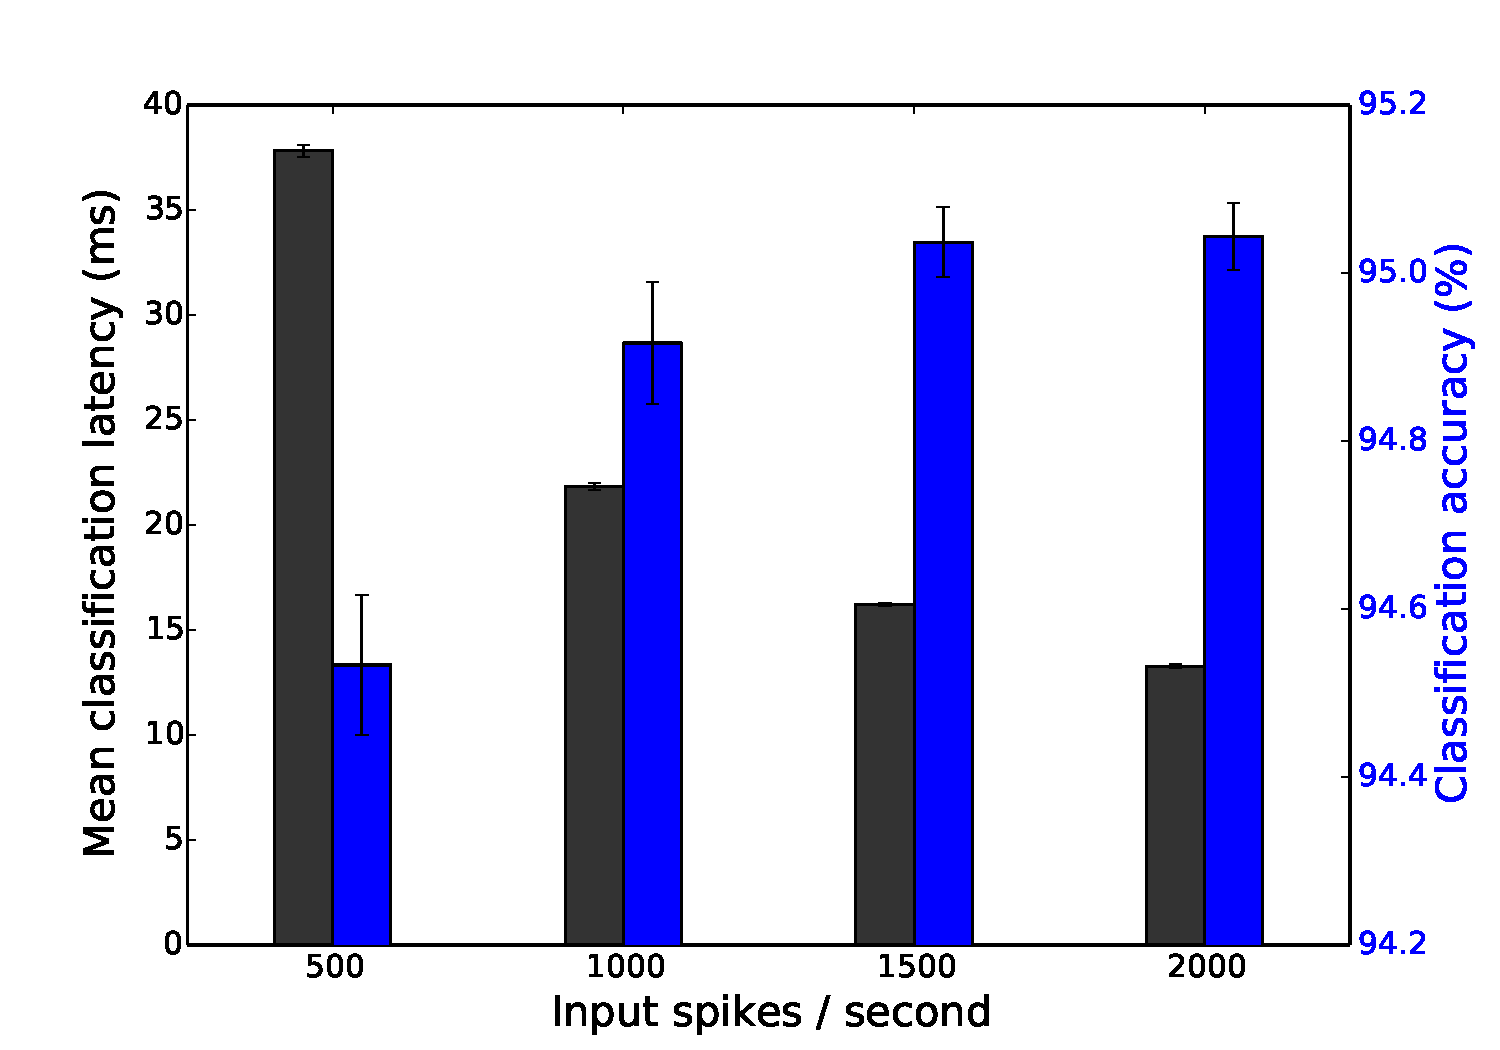
\includegraphics[width=0.48\textwidth]{images/evan/latencyCAfiringrate.pdf}
	\caption{Mean classification latency and classification accuracy as a function of the input spikes per second for the spiking DBN. Results are averaged over 4 trials, error bars show standard deviations.}
	\label{Fig:brianLatency}
\end{figure} 



\begin{figure}[hbt!]
	\centering
	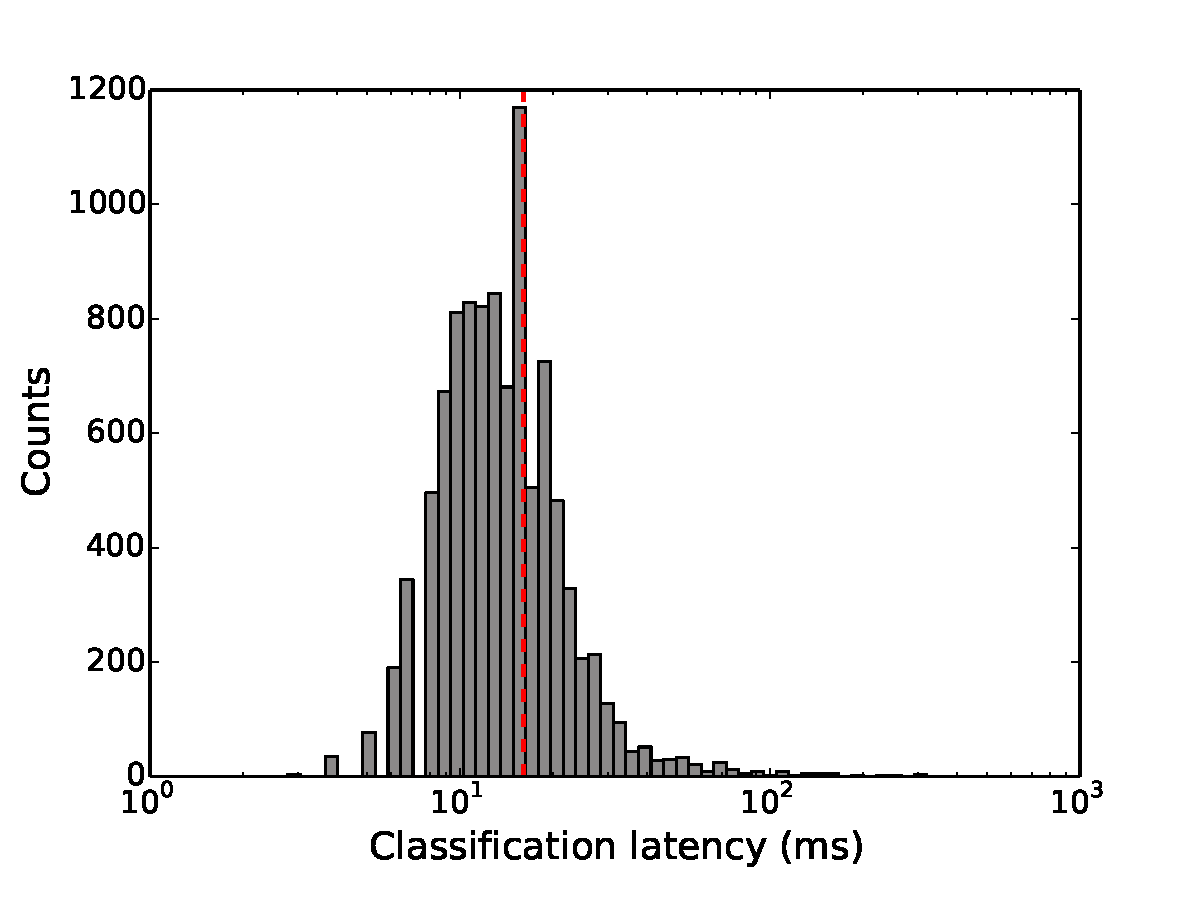
\includegraphics[width=0.48\textwidth]{images/evan/classlatencyIJCNN1500hz.pdf}
	\caption{Histogram of the classification latencies for the MNIST digits of the testing set when the input rates are set to 1500 Hz. The mean classification latency of the spiking DBN on SpiNNaker is 16 ms.}
	\label{Fig:spinnLatency1500hz}
\end{figure} 

%Mention power consumption and compare against an
%FPGA implementation on the identical network

Finally, this particular spiking DBN ran on a single SpiNNaker chip (16 ARM9 cores) and dissipated less than 0.3~W when 2000 spikes per second per digit were used, as seen in Figure~\ref{Fig:spinnchipPower}. The identical network ran on Minitaur \citep{dannminitaur}, an event-driven FPGA implementation, and consumed 1.5~W when 1000 spikes per image were used.  


\begin{figure}[hbt!]
	\centering
	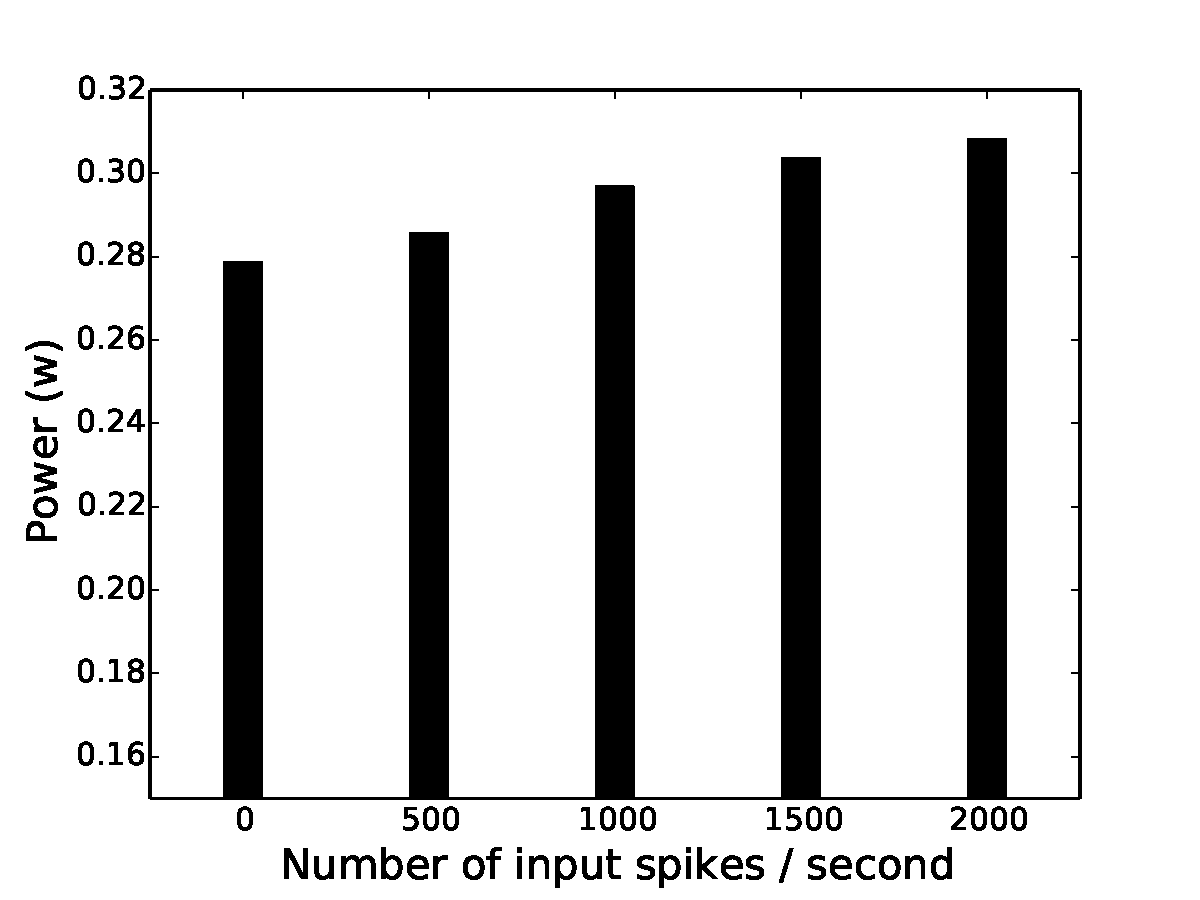
\includegraphics[width=0.48\textwidth]{images/evan/powerspinnaker.pdf}
	\caption{Power dissipation of a spiking DBN running on a single SpiNNaker chip as a function of the total number of input spikes per second.}
	\label{Fig:spinnchipPower}
\end{figure} 


%
%To investigate how the precision of the weights of an offline trained spiking DBN mapped 
%
%investigate how the weight precision and input firing rates affect the CA. 
%
%how input rates affect the classification latency
%
%results from spinnaker 
%table with CA
%latency from spinnaker
%
%
%\begin{figure}[hbt!]
%	\centering
%	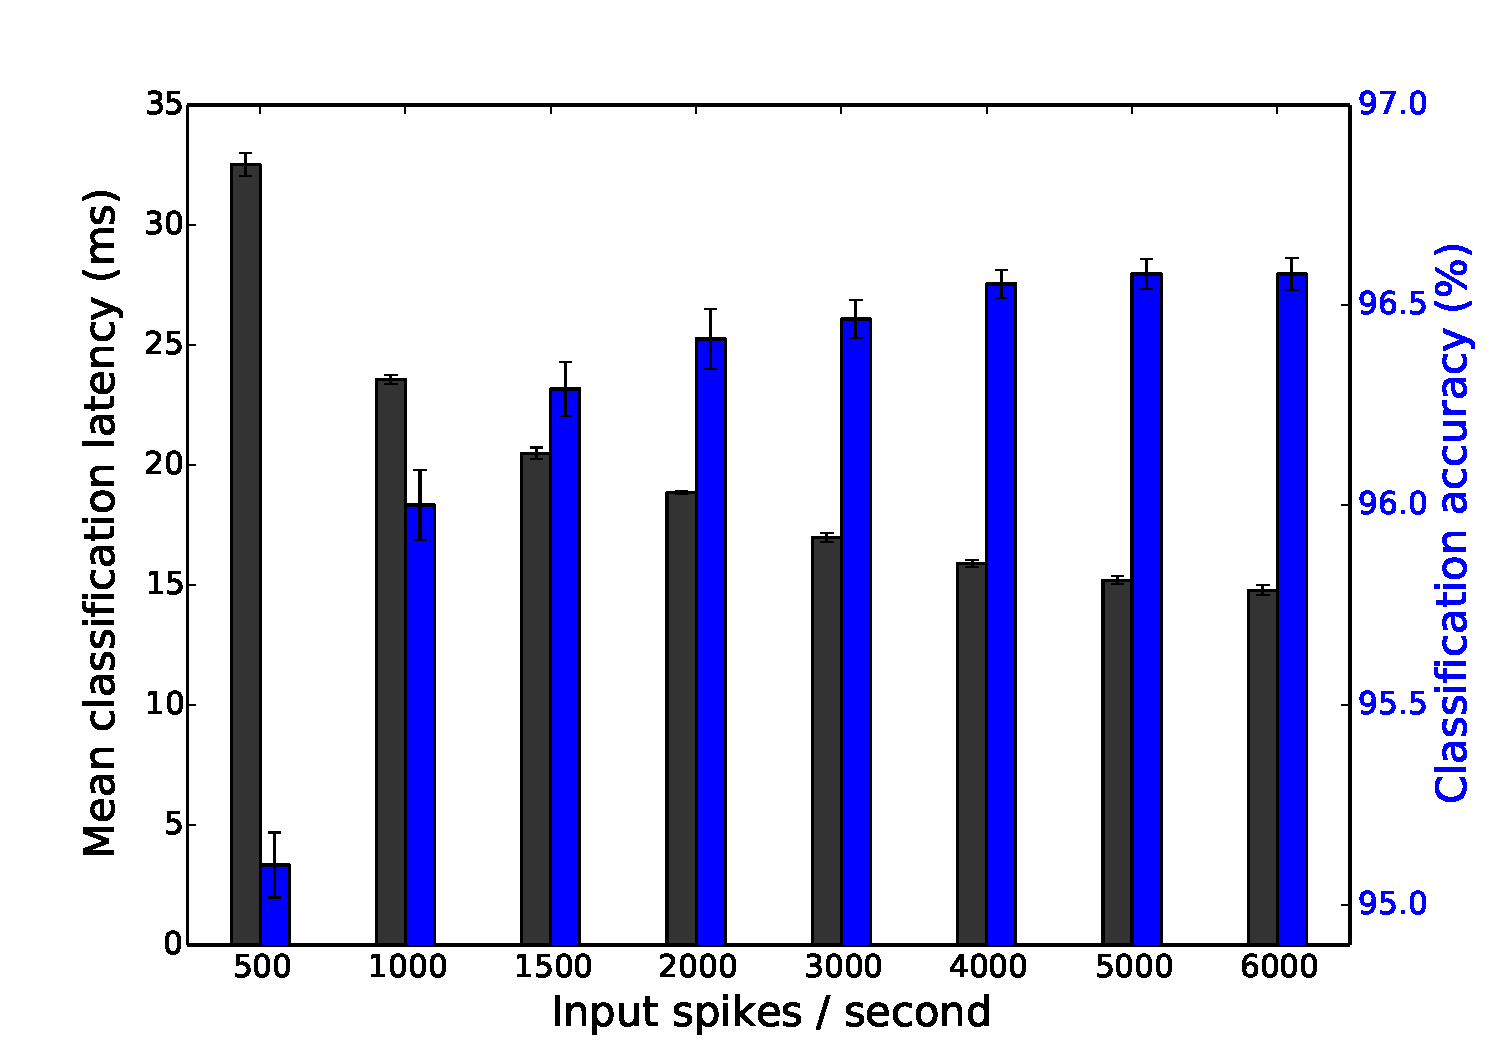
\includegraphics[width=0.48\textwidth]{images/evan/meanCAvsLatencyvsFiringrate_7hlayer.pdf}
%	\caption{Classification accuracy as a function of the input firing rates.}
%	\label{Fig:rateVSca}
%\end{figure} 
